%!TEX root = ../main.tex
\documentclass{beamer} % Gliederung im Kopf, sections und subsections
\renewcommand{\baselinestretch}{1.2}\normalsize
\usetheme{default}
\setbeamertemplate{navigation symbols}{}
\setbeamertemplate{footline}[frame number]

\usepackage{tabu}
\usepackage{etex}
%\usepackage{beamerthemesplit}
%\useoutertheme[subsection=false]{smoothbars}
%\usepackage[final]{pdfpages}
\usepackage{bibentry}
\usepackage{bm}
\usepackage{bigints}
\usepackage{graphicx}
\usepackage{relsize}
\usepackage[round,longnamesfirst]{natbib}
\usepackage{bm}																									%matrix symbol
\usepackage{bbm}

\usepackage{algpseudocode}
\usepackage{algorithmicx}
\usepackage{verbatim}
\usepackage{setspace}																					%Fu�noten (allgm.
\usepackage{hyperref}

\usepackage{bibentry}

\DeclareMathOperator*{\argmin}{arg\,min}
\DeclareMathOperator*{\argmax}{arg\,max}

\nobibliography*
\renewcommand{\vec}[1]{\mathbf{#1}}

\hypersetup{colorlinks=true,urlcolor=blue}														%Zeilenabst�nde)
\usepackage{threeparttable}
\usepackage{subfig}
\usepackage{epstopdf}
\usepackage{lscape}																							%Querformat
\usepackage[latin1]{inputenc}																		%Umlaute
\usepackage{graphicx}
\graphicspath{{../material/}}

\usepackage{booktabs}
\usepackage{amsmath}
\usepackage{amssymb}
%\usepackage{uarial}

\usepackage{tabularx}
\usepackage{fancybox}																						%Boxen und Rahmen
\usepackage{appendix}
\usepackage{enumerate}

%EURO Symbol
\usepackage{tabularx}
\usepackage{longtable}																					%Mehrseitige Tabellen
\usepackage{fix-cm}
\usepackage[T1]{fontenc}
\usepackage{color,colortbl}																			%Farbige Tabellen
\usepackage{threeparttable}
\usepackage{hyperref}
\usepackage{amsfonts}

\usepackage{graphicx}
\usepackage{caption}

\usepackage{tikz}
\tikzset{
  treenode/.style = {shape=rectangle, rounded corners,
                     draw, align=center,
                     top color=white, bottom color=blue!20},
  root/.style     = {treenode, font=\Large, bottom color=red!30},
  env/.style      = {treenode, font=\ttfamily\normalsize},
  dummy/.style    = {circle,draw}
}
%\usepackage{cmbright}
\def\newblock{\hskip .11em plus .33em minus .07em}
\newcommand{\bs}{\boldsymbol}
\newcommand{\N}{\mathbb{N}}
\newcommand{\cov}{\mathrm{cov}\thin}
\newcommand{\thin}{\thinspace}
\newcommand{\thick}{\thickspace}

\newcommand{\vect}[1]{\mathbf{#1}}
\newcommand{\myfrac}[3][0pt]{\genfrac{}{}{}{}{\raisebox{#1}{$#2$}}{\raisebox{-#1}{$#3$}}}
\newcommand{\U}{\mathrm{U}}	%Uniform Distribution
\newcommand{\D}{\mathrm{D}}	%Dirichlet Distribution
\newcommand{\W}{\mathrm{W}}	%Wishart Distribution
\newcommand{\E}{\mathrm{E}}		%Expectation
\newcommand{\Prob}{\mbox{Pr}}		%Expectation
\newcommand{\Iden}{\mathbb{I}}	%Identity Matrix
\newcommand{\Ind}{\mathrm{I}}	%Indicator Function
\newcommand{\Tau}{\mathcal{T}\thin}

\newcommand{\var}{\mathrm{var}\thin}
\newcommand{\plim}{\mathrm{plim}\thin}
\newcommand\indep{\protect\mathpalette{\protect\independenT}{\perp}}
\def\independenT#1#2{\mathrel{\rlap{$#1#2$}\mkern5mu{#1#2}}}
\newcommand{\notindep}{\ensuremath{\perp\!\!\!\!\!\!\diagup\!\!\!\!\!\!\perp}}%

\newcommand{\mc}{\multicolumn}

\newcommand{\ph}{\phantom}
% weitere Optionen:
% secbar: Gliederung im Kopf, nur sections (alternativ zu subsecbar)
% handout: Produktion von Handouts, keine Animationen
\definecolor{darkblue}{rgb}{0,.35,.62}
\definecolor{lightblue}{rgb}{0.8,0.85,1}
\definecolor{lightgrey}{gray}{0.1}	%Farben mischen

%	kbordermatrix options

\makeatletter
\newcommand{\vast}{\bBigg@{4}}
\newcommand{\Vast}{\bBigg@{5}}
\makeatother
\newcommand{\indicator}[1]{\mathbbm{1}{\left\{ {#1} \right\} }}
\newcommand{\indic}{1{\hskip -2.5 pt}\hbox{1} }


\definecolor{lightgrey}{gray}{0.90}	%Farben mischen
\definecolor{grey}{gray}{0.85}
\definecolor{darkgrey}{gray}{0.65}
\definecolor{lightblue}{rgb}{0.8,0.85,1}

\renewcommand{\arraystretch}{1.5}


\usepackage{tikz}
\usetikzlibrary{trees,shapes,arrows,decorations.pathmorphing,backgrounds,positioning,fit,petri}
\renewcommand*{\familydefault}{\sfdefault}

\tikzset{forestyle/.style = {rectangle, thick, minimum width = 5cm, minimum height = 0.5cm, text width = 4.5cm, outer sep = 1mm},
	pre/.style={<-, shorten <=1pt, >=stealth, ultra thick},
	extend/.style={<-,dashed, shorten <=1pt, >=stealth, ultra thick}}
\captionsetup[subfigure]{labelformat=empty}


\newcommand{\beginbackup}{
   \newcounter{framenumbervorappendix}
   \setcounter{framenumbervorappendix}{\value{framenumber}}
}
\newcommand{\backupend}{
   \addtocounter{framenumbervorappendix}{-\value{framenumber}}
   \addtocounter{framenumber}{\value{framenumbervorappendix}}
}


% Begin Full Justification ---------------------------------------------------------

\usepackage{ragged2e}
% \usepackage{etoolbox}
\usepackage{lipsum}
\makeatletter
\renewcommand{\itemize}[1][]{%
  \beamer@ifempty{#1}{}{\def\beamer@defaultospec{#1}}%
  \ifnum \@itemdepth >2\relax\@toodeep\else
    \advance\@itemdepth\@ne
    \beamer@computepref\@itemdepth% sets \beameritemnestingprefix
    \usebeamerfont{itemize/enumerate \beameritemnestingprefix body}%
    \usebeamercolor[fg]{itemize/enumerate \beameritemnestingprefix body}%
    \usebeamertemplate{itemize/enumerate \beameritemnestingprefix body begin}%
    \list
      {\usebeamertemplate{itemize \beameritemnestingprefix item}}
      {\def\makelabel##1{%
          {%
            \hss\llap{{%
                \usebeamerfont*{itemize \beameritemnestingprefix item}%
                \usebeamercolor[fg]{itemize \beameritemnestingprefix item}##1}}%
          }%
        }%
      }
  \fi%
  \beamer@cramped%
  \justifying% NEW
  %\raggedright% ORIGINAL
  \beamer@firstlineitemizeunskip%
}

\justifying

% \apptocmd{\frame}{\justifying}{}{}

\usepackage{array}
\newcolumntype{L}[1]{>{\raggedright\let\newline\\\arraybackslash\hspace{0pt}}m{#1}}
\newcolumntype{C}[1]{>{\centering\let\newline\\\arraybackslash\hspace{0pt}}m{#1}}
\newcolumntype{R}[1]{>{\raggedleft\let\newline\\\arraybackslash\hspace{0pt}}m{#1}}



% End Full Justification ------------------------------------------------------------

%!TEX root = ../main.tex
\title{Generalized Roy Model}
\author{Philipp Eisenhauer}

\date{}

\let\otp\titlepage
%\renewcommand{\titlepage}{\otp\addtocounter{framenumber}{-1}}

\begin{document}
\maketitle

\begin{frame}


\begin{itemize}
\item Does the pursuit of comparative advantage increase or decrease earnings in equality within sectors and in the overall economy?
\item Do the people with the highest $i$ skill actually work in sector $i$?
\item As people enter a sector in response to an increase in the demand for its services, does the average skill level employed there rise or fall?
\end{itemize}

\end{frame}


\begin{frame}
\textbf{\citet{Roy.1951} Model}
\begin{itemize}
\item Individuals are income maximizing, act under perfect information, and possess skills $S_1$ and $S_2$.
\item The economy offers two employment opportunities associated with skill prices $\pi_1$ and $\pi_2$ and skill $i$ is only useful in sector $i$.
\end{itemize}\vspace{0.5cm}

An individual chooses sector one if earnings are greater there:
\begin{align*}
w_1 > w_2 \quad\Longleftrightarrow\quad \pi_1 S_1 > \pi_2 S_2
\end{align*}
\end{frame}


\begin{frame}
\textbf{Econometric Problems}

\begin{itemize}
\item \textbf{Evaluation Problem} We only observe an individual's wage in the sector they are working in.
\item \textbf{Selection Problem} As individuals pursue their comparative advantage, we only observe selected samples from the latent skill distribution in either sector.
\end{itemize}\vspace{0.5cm}


\end{frame}



\begin{frame}
\textbf{Key Questions}\\
\begin{itemize}\setlength\itemsep{1em}
\item What economic concepts are accounted for, which are not?
\item What does the individual, what does the econometrician know?
\item What gives rise to heterogeneity in skills?
\end{itemize}
\end{frame}


\begin{frame}
\begin{itemize}
\item Skills follow a bivariate normal distribution denoted by $F(s_1, s_2)$.
\end{itemize}

\begin{align*}
\begin{pmatrix}
 \ln S_1 \\
 \ln S_2
\end{pmatrix}  \sim \mathcal{N} \left( \begin{pmatrix}
 \mu_1 \\
 \mu_2
\end{pmatrix} , \begin{pmatrix}
 \sigma^2_1  &  \sigma_{12} \\
 \sigma_{21}&  \sigma^2_2
\end{pmatrix} \right)
\end{align*}

\end{frame}

\begin{frame}
\begin{figure}[htp]\centering
\caption{Joint Distribution of Skills}\label{Joint Distribution of Skills}\scalebox{0.35}{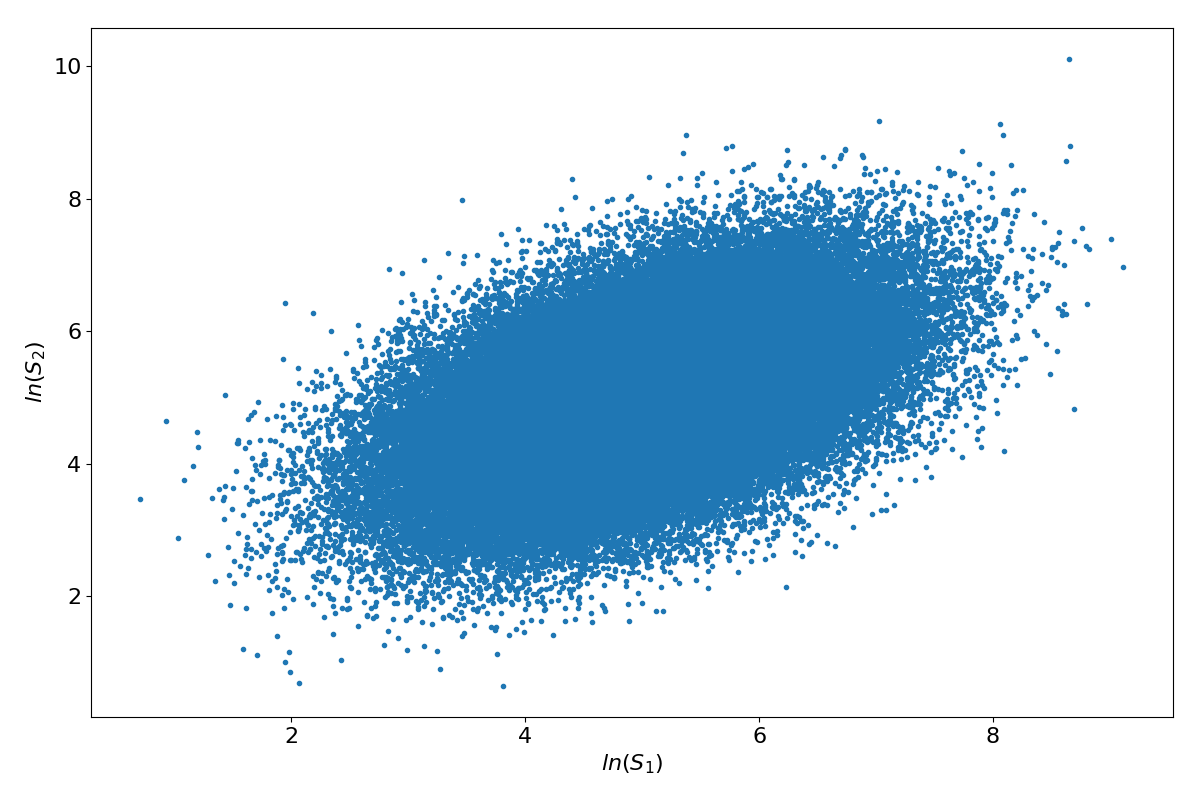
\includegraphics{fig-distribution-skills-latent-joint}}
\end{figure}
\end{frame}

\begin{frame}
\begin{figure}[htp]\centering
\caption{Marginal Distribution of Skill}\label{Marginal Distribution of Skill}\scalebox{0.35}{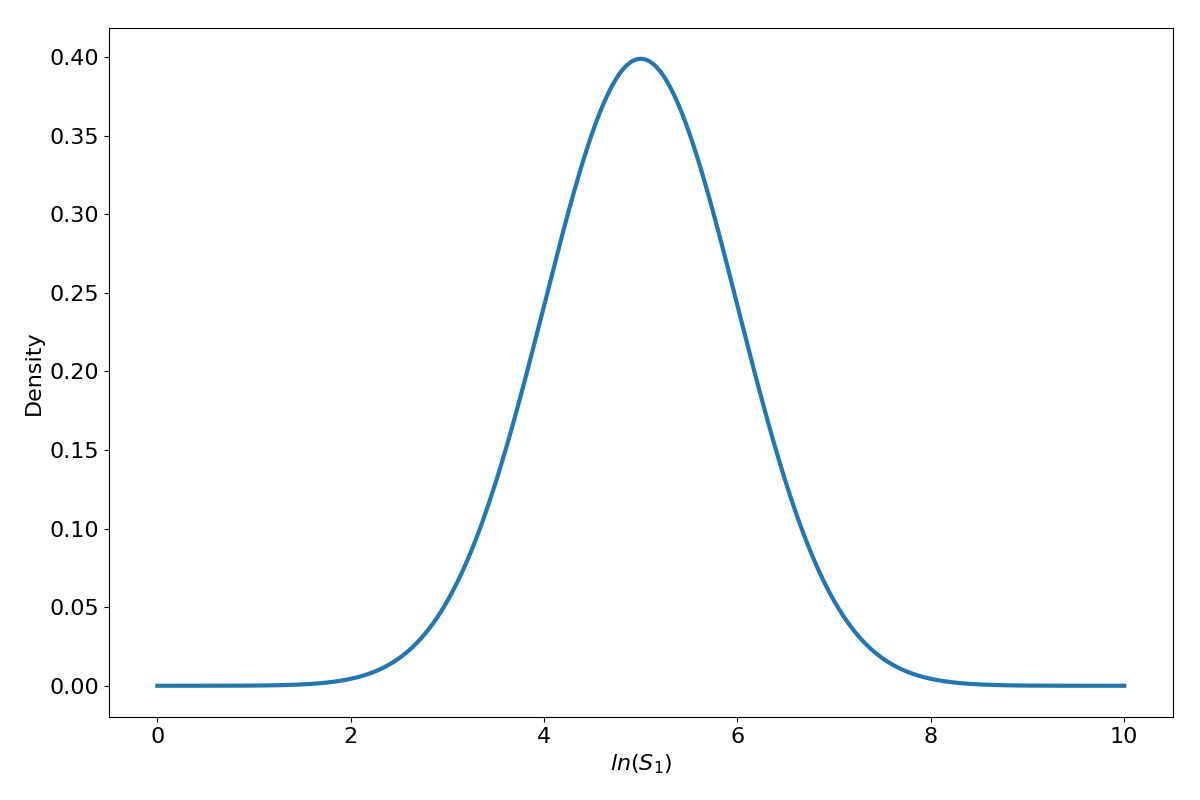
\includegraphics{fig-distribution-skills-latent-marginal}}
\end{figure}
\end{frame}


 \begin{frame}
 The proportion of the population working in sector one $P_1$
 \begin{align*}
 P_1 = \int^\infty_0 \int^{\pi_1 s_1 / \pi_2}_0 f(s_1, s_s) ds_1ds_2
 \end{align*}

 The density of skills employed in sector one differs from the population density of skills.

 \begin{align*}
 f(s_1) & = \int^\infty_0 f(s_1, s_2) ds_2 \\
 g_1(s_1 \mid \pi_1 S_1 > \pi_2 S_2) & = \frac{1}{P} \int^{\pi_1 s_1 /\pi_2}_0 f(s_1, s_2) ds_2
 \end{align*}


 The distribution of skills employed in sector $i$ differs from the population distribution of skills due to comparative advantage.
 \end{frame}



\begin{frame}
\begin{figure}[htp]\centering
\caption{Latent and Observed Distribution of Skill}\label{Latent and Observed Distribution of Skill}\scalebox{0.35}{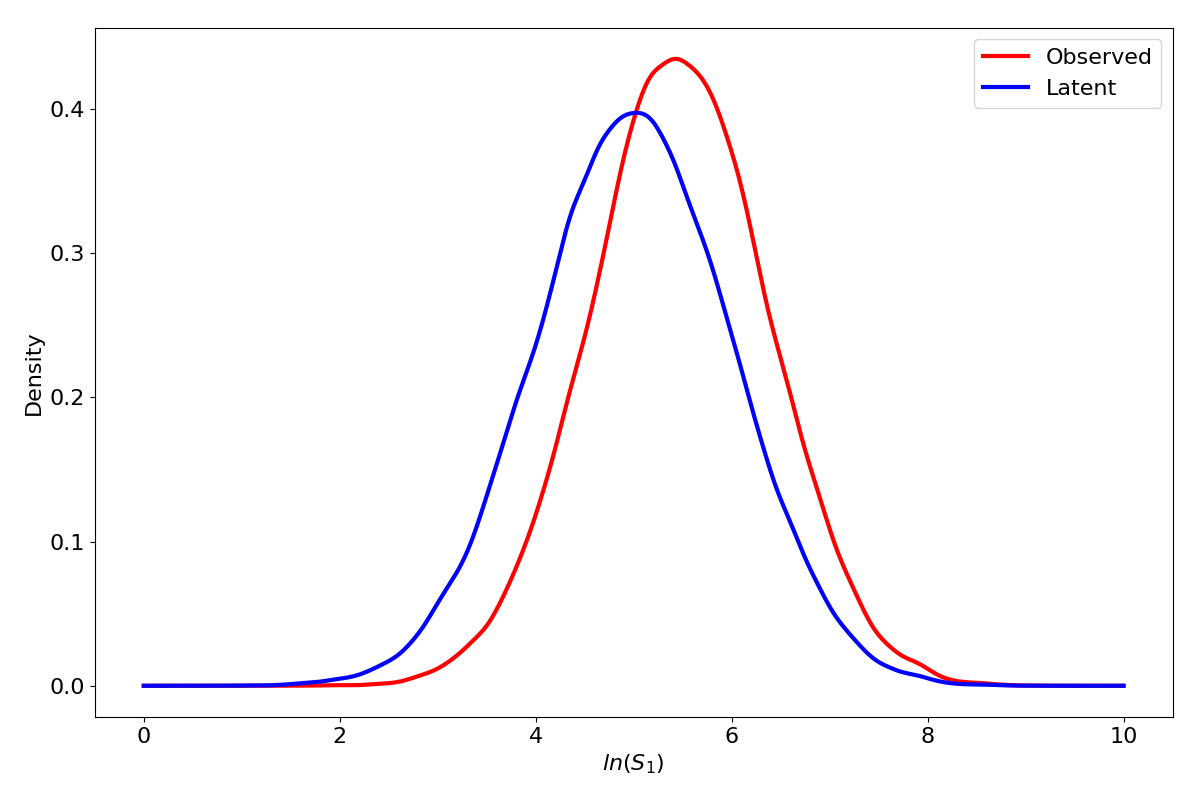
\includegraphics{fig-distribution-skills-both-marginal}}
\end{figure}
\end{frame}


\begin{frame}

\textbf{Wage Equations}

\begin{align*}
\ln W_1 & = \ln \pi_1 + \mu_1 + U_1 \\
\ln W_2 & = \ln \pi_2 + \mu_2 + U_2, \\
\end{align*}
where $U_i = \ln S_i - \mu_i$.

\end{frame}


\begin{frame}

\textbf{Sorting}

\begin{align*}
E[\ln S_1 \mid \ln W_1 > \ln W_2] & = \mu_1 + \frac{\sigma_{11} - \sigma_{12}}{\sigma^*} \lambda(-c_1) \\
E[\ln S_2 \mid \ln W_2 > \ln W_1] & = \mu_2 + \frac{\sigma_{22} - \sigma_{12}}{\sigma^*} \lambda(-c_2)
\end{align*}

We know the following:

\begin{align*}
\sigma^2 = (\sigma_{11} - \sigma_{12}) -  (\sigma_{22} - \sigma_{12}) > 0
\end{align*}

\begin{itemize}
\item There must be positive selection into one of the occupations and there can be positive selection into both.
\end{itemize}

\end{frame}


\begin{frame}
\begin{figure}[htp]\centering
\caption{Marginal Distributions of Skills}\label{Marginal Distributions of Skills}\scalebox{0.35}{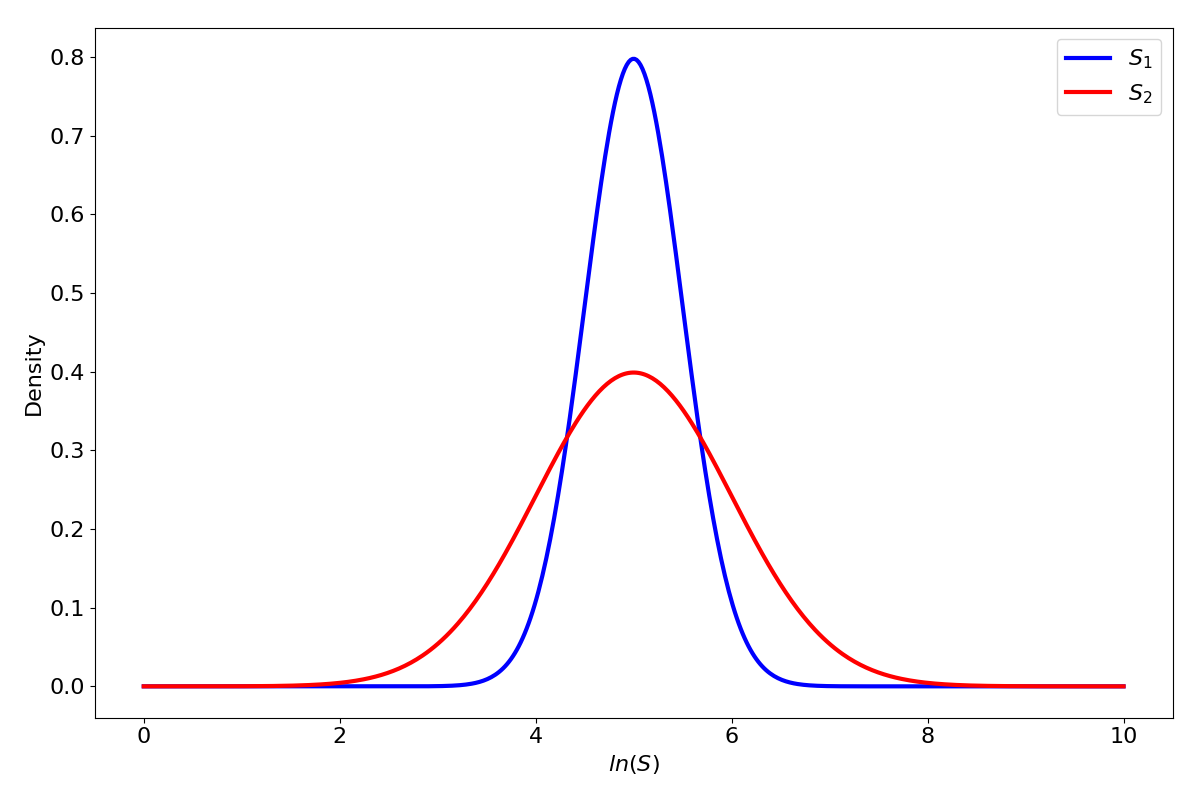
\includegraphics{fig-distribution-skills-latent-marginal-two.png}}
\end{figure}
\end{frame}



\begin{frame}
\textbf{What do we know?}
\begin{itemize}\setlength\itemsep{1em}
\item There is positive selection in Sector 2, because there cannot be negative selection in both and $\sigma_{22} > \sigma_{11}$.
\end{itemize}\vspace{0.5cm}

\textbf{How about Sector 1?}
\begin{itemize}\setlength\itemsep{1em}
\item If $\sigma_{12} < 0$, then there is also positive selection in Sector 1.
\item If $\rho_{12} = 1$, then there is negative selection into Sector 1 as $\sigma_{12} > \sigma_{11}$
\end{itemize}

\end{frame}



%-------------------------------------------------------------------------------
%-------------------------------------------------------------------------------
\begin{frame}\begin{center}
\LARGE\textit{Importance of Assignment Mechanism}
\end{center}\end{frame}
%-------------------------------------------------------------------------------
%-------------------------------------------------------------------------------

\begin{frame}

\citet{Heckman.1990} show that ... \vspace{0.5cm}

\begin{quote} For a log normal Roy economy, any random assignment of persons to sectors with the same proportion of persons in each sector as in the Roy economy has higher variance of log earnings provided the proportions lie strictly in the unit interval. This is true whether or not skill prices in the two economies are the same.
\end{quote}
\end{frame}

\begin{frame}
\begin{center} \textbf{Choices over Time}\\\vspace{0.5cm}
\scalebox{0.6}{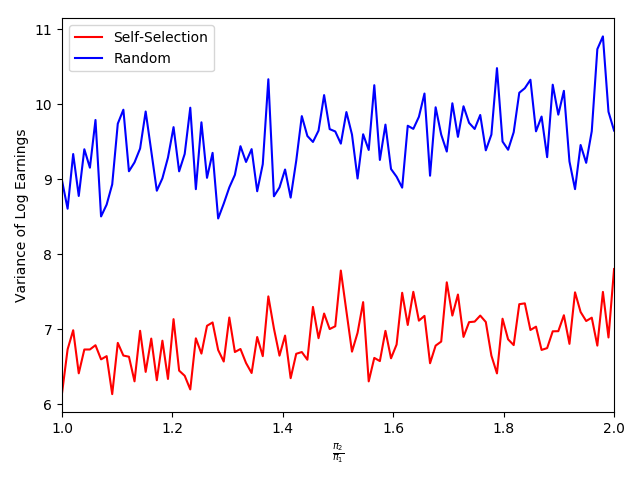
\includegraphics{fig-assignment-mechanism.png}}
\end{center}
\end{frame}

%-------------------------------------------------------------------------------
%-------------------------------------------------------------------------------
\begin{frame}\begin{center}
\LARGE\textit{Incarnations of the Roy Model}
\end{center}\end{frame}
%-------------------------------------------------------------------------------
%-------------------------------------------------------------------------------
\begin{frame}
\textbf{The Generalized Roy Model}

\begin{align*}
\text{Potential Outcomes} &\qquad \text{Cost} \\
Y_1 = \mu_1(X) + U_1      &\qquad C = \mu_D(Z) + U_C \\
Y_0 = \mu_0(X) + U_0      &\qquad \\
    & \\
\text{Observed Outcomes } &\qquad \text{Choice} \\
Y = D Y_1 + (1 - D)Y_0 &\qquad S = Y_1 - Y_0 - C \\
                       &\qquad D = \mathrm{I}[S > 0] \\
\end{align*}
\end{frame}

\begin{frame}
\begin{figure}[htp]\centering
\caption{Occupational Sorting in the Generalized Roy Model}\label{Occupational Sorting in the Generalized Roy Model}\scalebox{0.35}{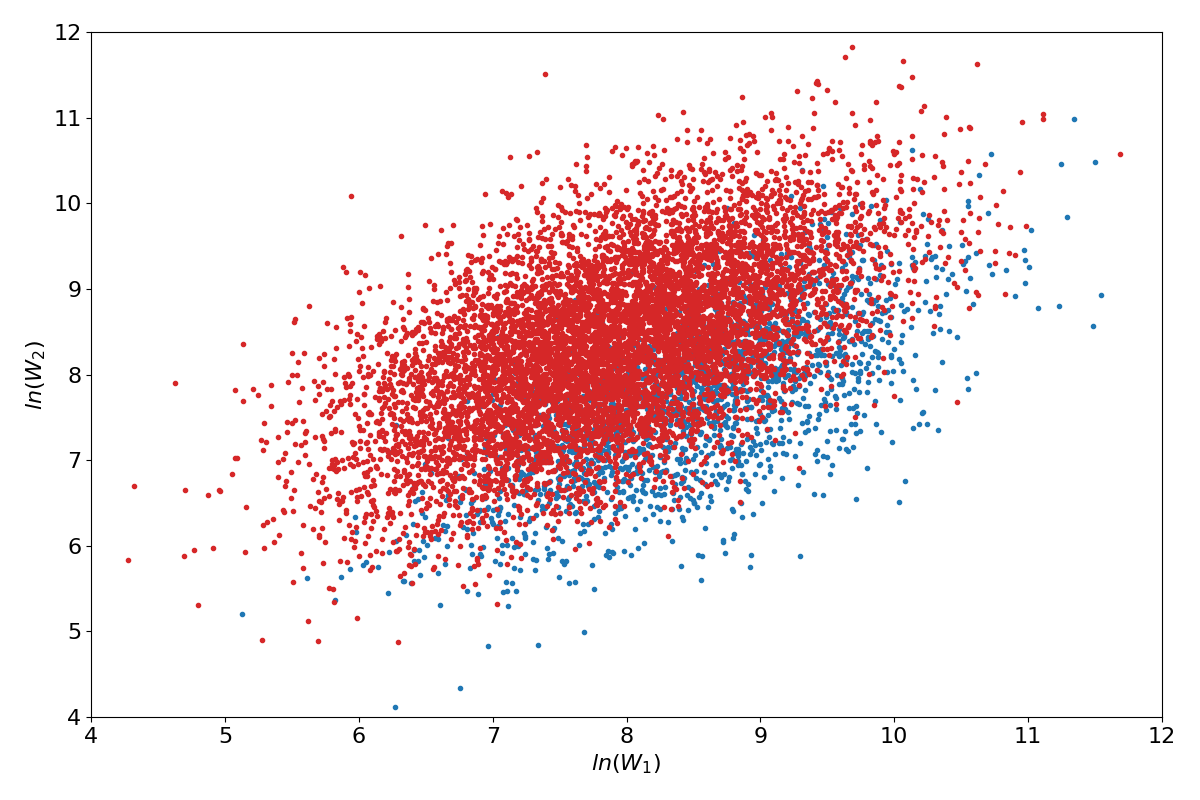
\includegraphics{fig-occupational-choices-generalized.png}}
\end{figure}
\end{frame}


\begin{frame}
\textbf{Extended Roy Model}

\begin{align*}
\text{Potential Outcomes} &\qquad \text{Cost} \\
Y_1 = \mu_1(X) + U_1      &\qquad C = \mu_D(Z) \\
Y_0 = \mu_0(X) + U_0      &\qquad \\
    & \\
\text{Observed Outcomes } &\qquad \text{Choice} \\
Y = D Y_1 + (1 - D)Y_0 &\qquad S = Y_1 - Y_0 - C \\
                       &\qquad D = \mathrm{I}[S > 0] \\
\end{align*}

\end{frame}




\begin{frame}
\begin{figure}[htp]\centering
\caption{Occupational Sorting in the Extended Roy Model}\label{Occupational Sorting in the Extended Roy Model}\scalebox{0.35}{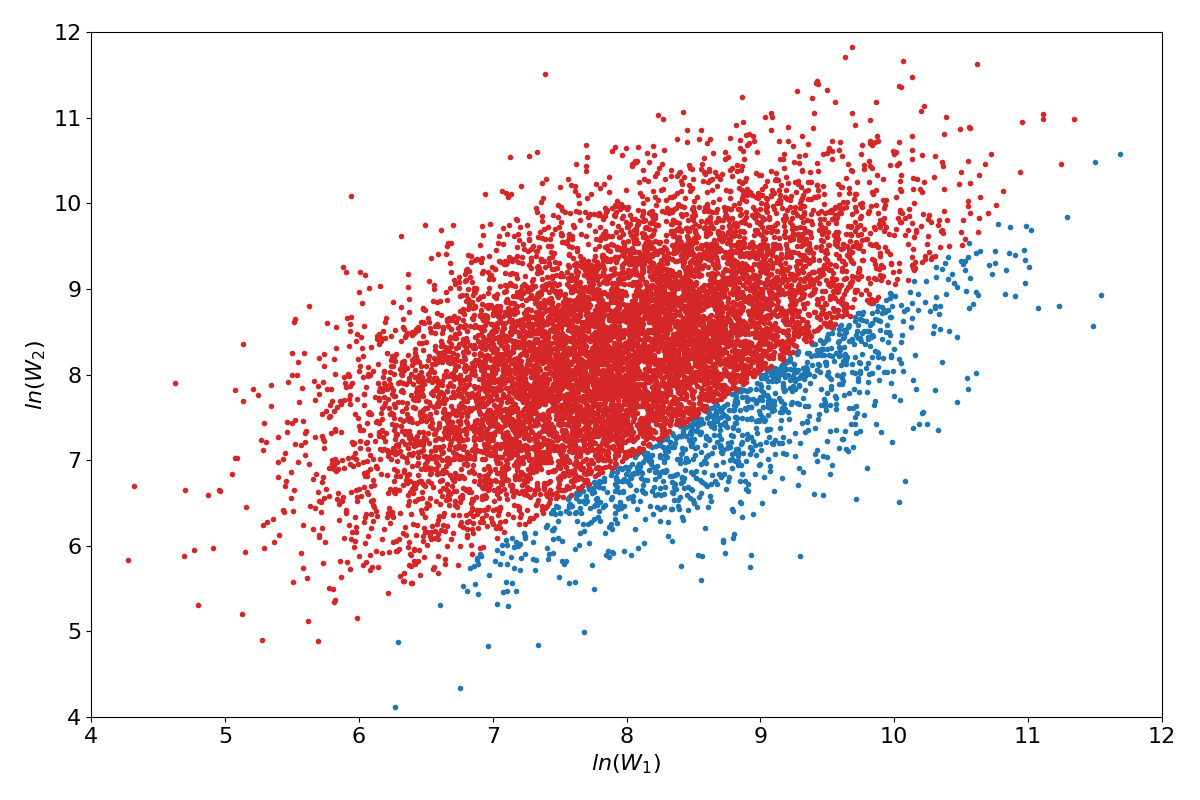
\includegraphics{fig-occupational-choices-extended.png}}
\end{figure}
\end{frame}




\begin{frame}
\textbf{Mapping Notation to original Roy Model}

\begin{align*}
\text{Potential Outcomes} &\qquad \text{Cost} \\
W_1 = \pi_1 S_1      &\qquad C = 0 \\
W_2 = \pi_2 S_2       &\qquad \\
    & \\
\text{Observed Outcomes } &\qquad \text{Choice} \\
W = D W_1 + (1 - D)W_2 &\qquad S = W_1 - W_2 \\
                       &\qquad D = \mathrm{I}[S > 0] \\
\end{align*}
\end{frame}

\begin{frame}
\begin{figure}[htp]\centering
\caption{Occupational Sorting in the Original Roy Model}\label{Occupational Sorting in the Original Roy Model}\scalebox{0.35}{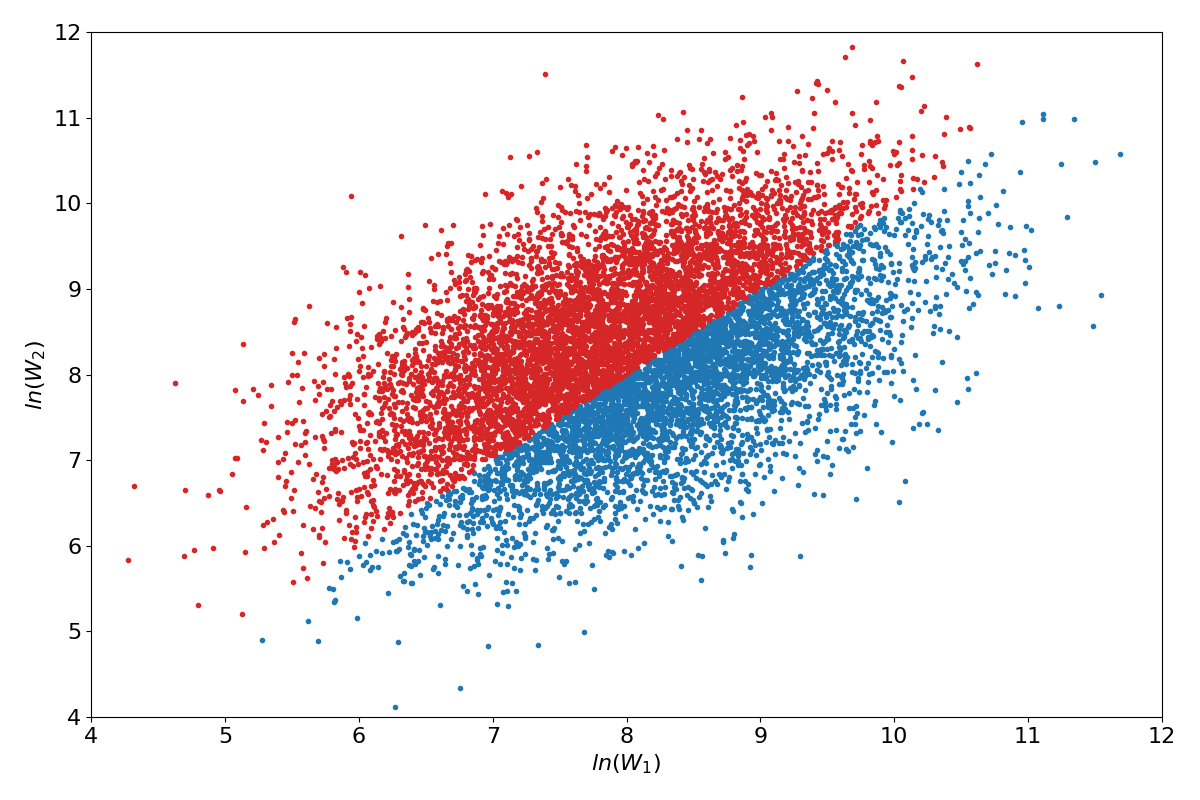
\includegraphics{fig-occupational-choices-original.png}}
\end{figure}
\end{frame}


%!TEX root = ../main.tex
\beginbackup\appendix
\begin{frame}\begin{center}
\LARGE\textbf{Appendix}
\end{center}\end{frame}

%------------------------------------------------------------------------------
%------------------------------------------------------------------------------
\begin{frame}\begin{center}
\LARGE\textit{References}
\end{center}\end{frame}
%------------------------------------------------------------------------------
%------------------------------------------------------------------------------
\newgeometry{margin=1cm}
\begin{frame}[allowframebreaks]\frametitle{}

\nocite{Carneiro.2011}

\bibliographystyle{apalike}
\bibliography{../../../submodules/bibliography/literature}


\end{frame}

\backupend
\end{document}
